\section{Beyond one-step models: predictive representations}
\label{sec:beyond}
\label{sec:successor}


The ``world models'' we described in \cref{sec:WM}
are \keywordDef{one-step models} of the form $p(s'|s,a)$,
or $p(z'|z,a)$ for $z=\phi(s)$, where $\phi$ is a state-abstraction
function.
However, such models are problematic when it comes to predicting
many kinds of future events, such as ``will a car pull in front of me?''
or ``when will it start raining?'',
since it is hard to predict exactly when these events will occur,
and these events may correspond to many different ``ground states''.
In principle we can roll out many possible long term futures,
and apply some abstraction function to  the resulting
generated trajectories to extract features of interest,
and thus derive a predictive model of the form $p(t', \phi(s_{t+1:t'})|s_t,\pi)$,
where $t'$ is the random duration of the sampled trajectory.
However, it would be more
efficient if we could directly predict this distribution
without having to know the value of $t'$,
and without having to predict all the details of all the
intermediate future states,
many of which will be irrelevant given the abstraction function $\phi$.
This motivates the study of multi-step world models,
that predict multiple steps into the future,
either at the state level, or at the feature level.
These are called \keywordDef{predictive representations},
and are a compromise between standard model-based RL
and model-free RL, as we will see.
Our presentation on this topic is based on 
\citep{Carvalho2024}.
% https://julien-vitay.net/post/successor_representations/
(See also \cref{sec:HRL}, where we discuss the related topic
of temporal abstraction from a model-free perspective.)

\subsection{General value functions}
\label{sec:GVF}

The value function is based on  predicting the sum of expected
discounted future rewards.
But the reward is just one possible signal of interest we can extract from the environment.
We can generalize this by considering a \keywordDef{cumulant}
$C_t \in \real$, which is some scalar of interest derived from the state or observation
(e.g., did a loud bang just occur? is there a tree visible in the image?).
We then define the \keywordDef{general value function} or \keywordDef{GVF}
as follows \citep{GVF}:
\be
V^{\pi,C,\gamma}(s) = \expect{
  \sum_{t=0}^{\infty} \gamma^t C(s_{t+1}) \vert s_0=s, a_{0:\infty} \sim \pi}
\ee
If $C(s_{t+1})=R_{t+1}$, this reduces to the value function.\footnote{
%
This follows the convention  of \citep{Suttonv2},
where we write $(s_t, a_t, r_{t+1}, s_{t+1})$
to represent the transitions, since
$r_{t+1}$ and $s_{t+1}$ are both generated
by applying $a_t$ in state $s_t$.
}
However, we can also define the GVF to predict components
of the observation vector; this is called \keywordDef{nexting} \citep{Modayil2014},
since it refers to next state prediction at different timescales.

\subsection{Successor representations}
\label{sec:SR}
\label{sec:PSR}


In this section we consider a variant of GVF
where the cumulant corresponds
to a state occupancy vector $C(s_{t+1}) = \ind{s_{t+1}=\tilde{s}}$,
which provides a dense feedback signal.
This give us the \keywordDef{successor representation} or \keywordDef{SR}
\citep{Dayan1993}:
\be
M^{\pi}(s,\tilde{s}) = \expect{
  \sum_{t=0}^{\infty} \gamma^t \ind{s_{t+1}=\tilde{s}} \vert S_0=s}
\ee
If we define the policy-dependent state-transition matrix by
\be
T^{\pi}(s,s') = \sum_a \pi(a|s) T(s'|s,a)
\ee
then the SR matrix can be rewritten as
\be
\vM^{\pi} = \sum_{t=0}^{\infty} \gamma^t [\vT^{\pi}]^{t+1}
= \vT^{\pi} (\vI - \gamma \vT^{\pi})^{-1}
\ee
Thus we see that the SR replaces information about
individual transitions with their cumulants,
just as the value function replaces individual rewards
with the reward-to-go.

Like the value function, the SR obeys a Bellman equation
\begin{align}
  M^{\pi}(s,\tilde{s})
  &= \sum_a \pi(a|s) \sum_{s'}
T(s'|s,a)\left( \ind{s'=\tilde{s}} + \gamma M^{\pi}(s',\tilde{s})
\right) \\
   &= \expect{\ind{s'=\tilde{s}} + \gamma M^{\pi}(s',\tilde{s})}
\end{align}
Hence we can learn an SR using a TD update of the form
\begin{align}
  M^{\pi}(s,\tilde{s}) &\leftarrow
  M^{\pi}(s,\tilde{s}) + \eta 
  \underbrace{\left( \ind{s'=\tilde{s}} + \gamma M^{\pi}(s',\tilde{s})
     - M^{\pi}(s,\tilde{s}) \right)}_{\delta}
\end{align}
where $s'$ is the next state sampled from $T(s'|s,a)$.
Compare this to the value-function TD update
in \cref{eqn:rl-td}:
\be
V^{\pi}(s) \leftarrow
V^{\pi}(s) + \eta \underbrace{ \left(
  R(s') + \gamma V^{\pi}(s') - V^{\pi}(s) \right)}_{\delta}
\ee
However, with an SR,
we can easily compute the value
function for any reward function
(as approximated by a given policy)
as follows:
\be
V^{R,\pi} = \sum_{\tilde{s}} M^{\pi}(s,\tilde{s}) R(\tilde{s})
\ee
See \cref{fig:successorRep} for an example.

\begin{figure}
\centering
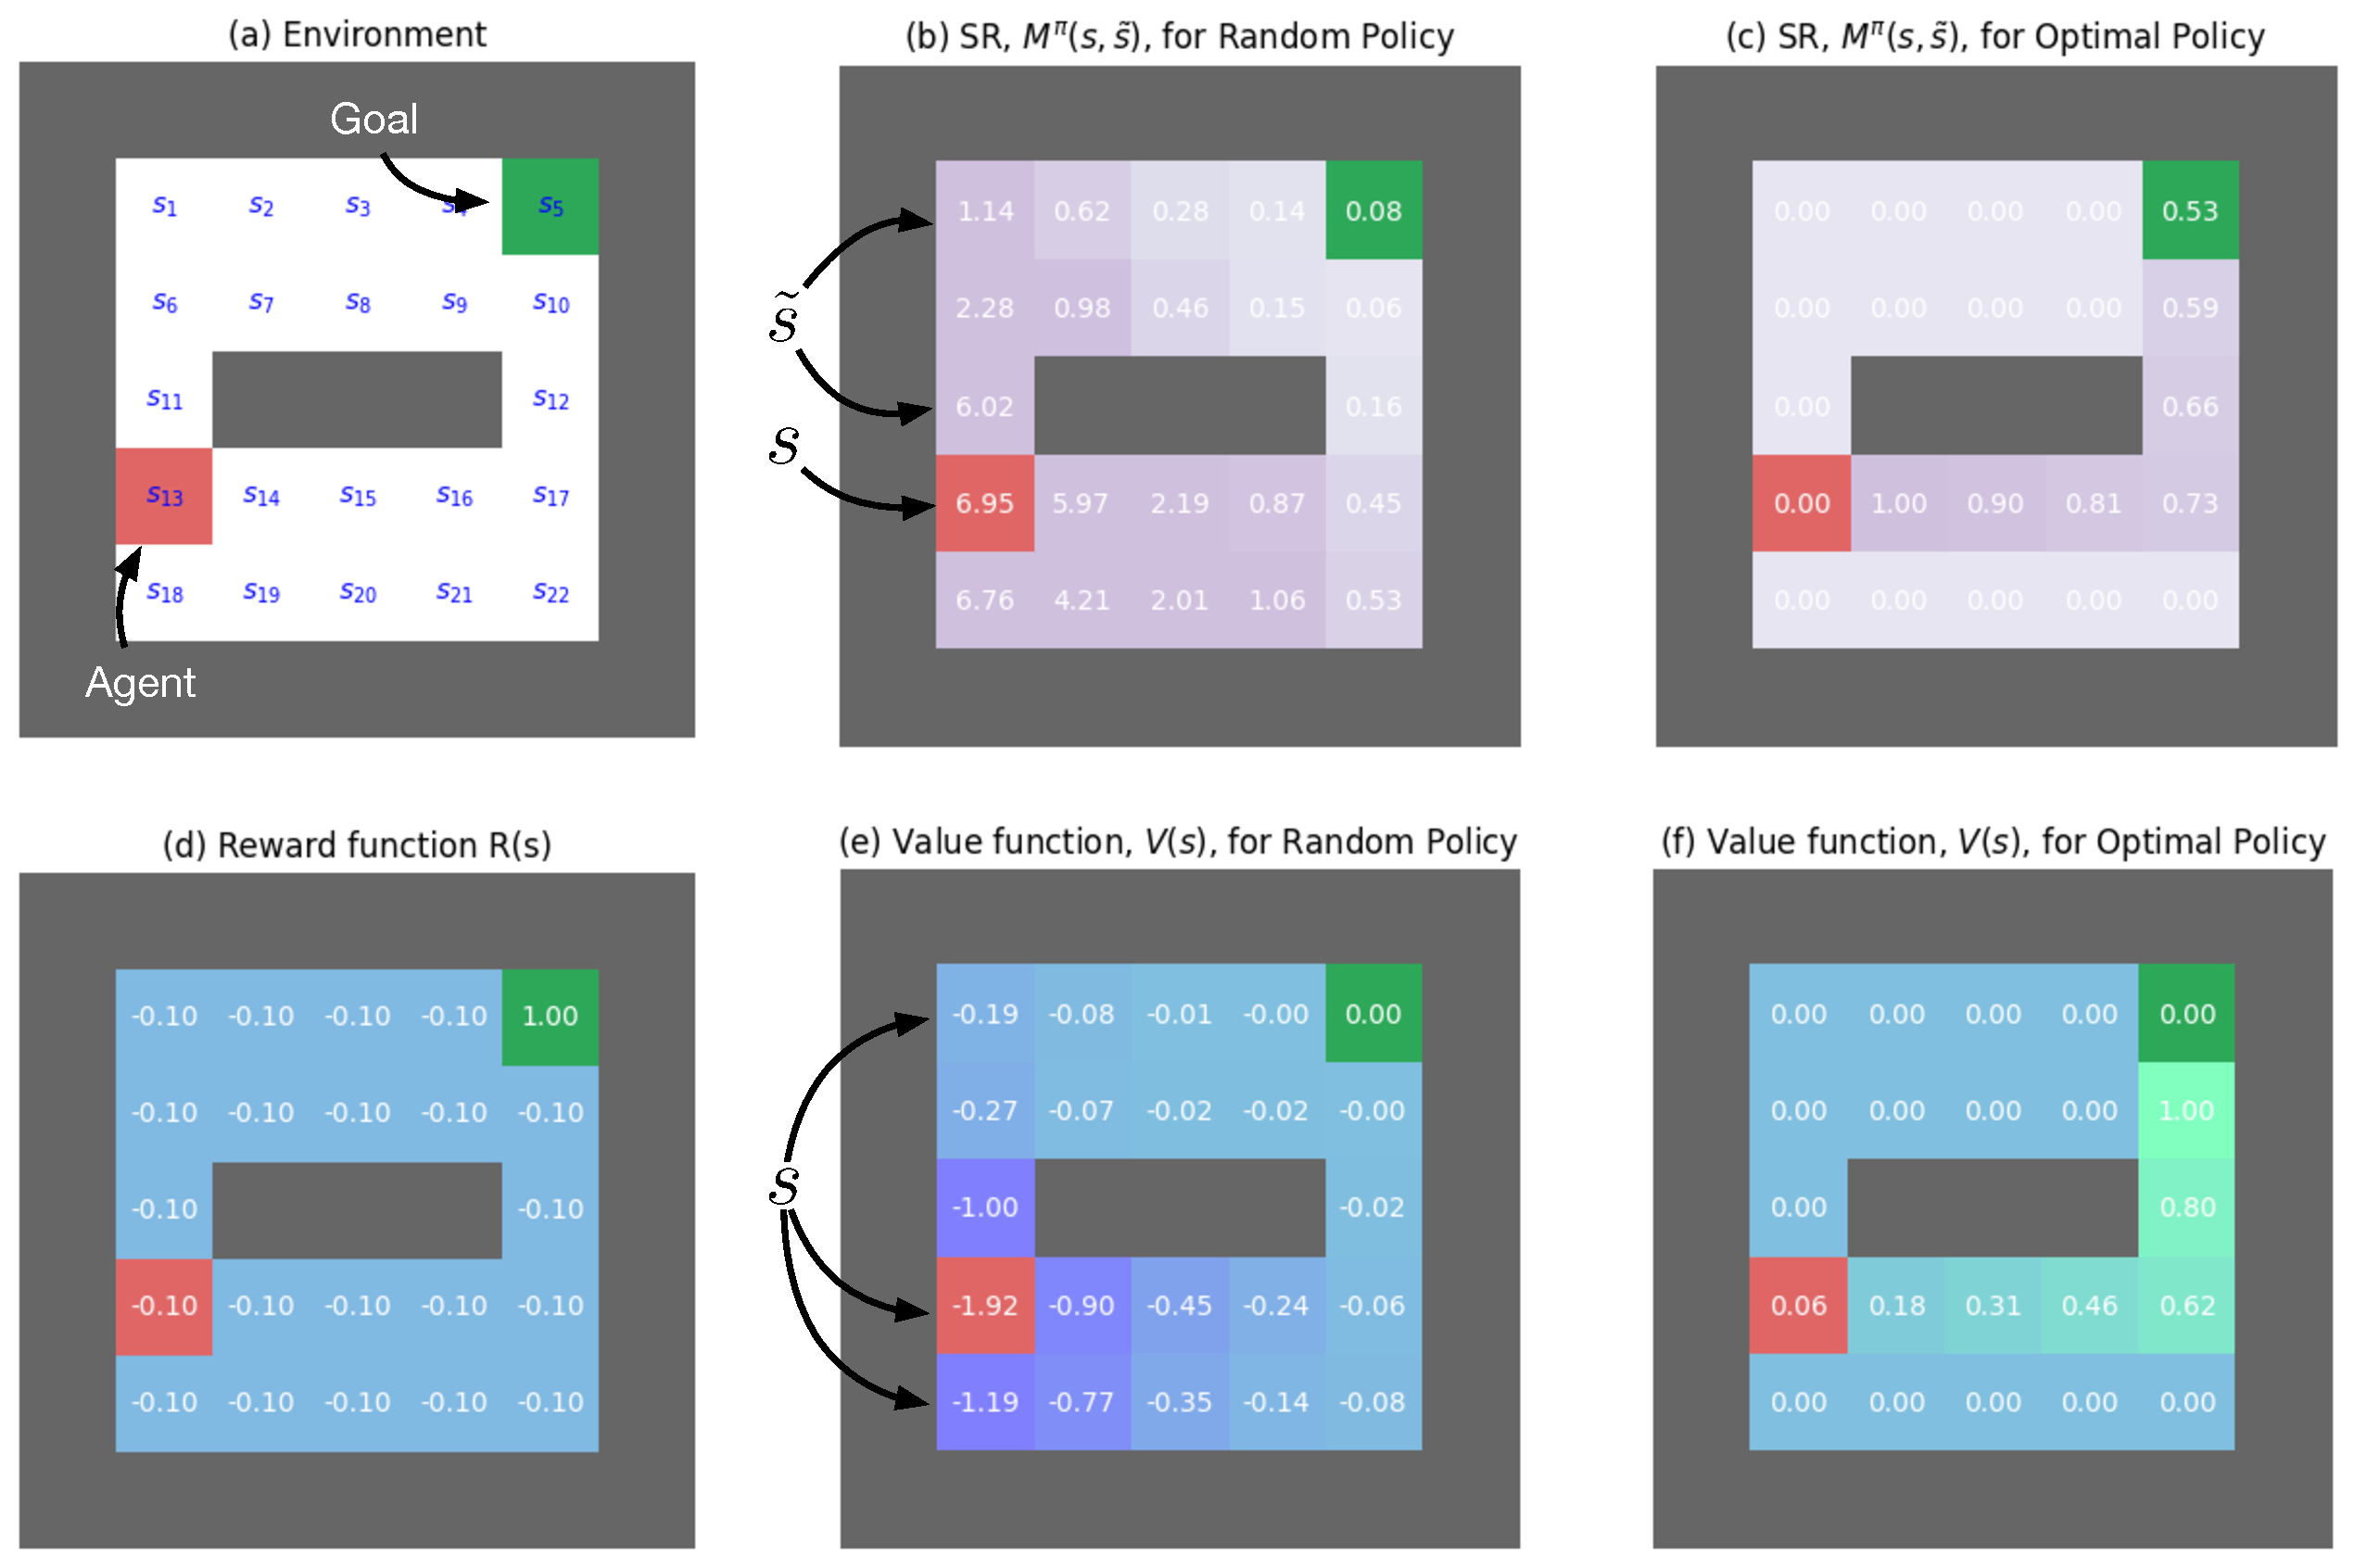
\includegraphics[height=3in]{figs/successor-rep}
\caption{
  % https://colab.sandbox.google.com/drive/1IxBmFARYobb1D3e26XzeSkTEOFxt8cxI?usp=sharing
  Illustration of successor representation for
  the 2d maze environment shown in (a) with reward
  shown in (d), which assings all states a reward of -0.1
  except for the goal state which has a reward of 1.0.
  In (b-c) we show the  SRs for a random policy and the optimal policy.
  In (e-f) we show the corresponding value functons.
%
  In (b), we see that the SR under the random policy
  assigns high state occupancy values to states which are close
  (in Manhattan distance)
  to the current state $s_{13}$
  (e.g., $M^{\pi}(s_{13}, s_{14})=5.97$)
  and low values to states that are further away
  (e.g., $M^{\pi}(s_{13}, s_{12})=0.16$).
%
  In (c), we see that the SR under the optimal policy
  assigns high state occupancy values to states which are close
  to the optimal path to the goal
  (e.g., $M^{\pi}(s_{13}, s_{14})=1.0$)
  and which fade with distance from the current state
  along that path
  (e.g., $M^{\pi}(s_{13}, s_{12})=0.66$).
  \figtaken{Figure 3 of \citep{Carvalho2024}}.
  \figthanks{Wilka Carvalho}.
  \figgen{\url{https://github.com/wcarvalho/jaxneurorl/blob/main/successor_representation.ipynb}}.
}
\label{fig:successorRep}
\end{figure}

We can also make a version of SR that depends on the action
as well as the state to get
\begin{align}
M^{\pi}(s,a,\tilde{s})
&= \expect{\sum_{t=0}^{\infty} \gamma^t \ind{s_{t+1}=\tilde{s}}
  \vert s_0=s, a_0=a, a_{1:\infty} \sim \pi} \\
&= \expect{\ind{s'=\tilde{s}} + \gamma M^{\pi}(s',a,\tilde{s})
  \vert s_0=s, a_0=a, a_{1:\infty} \sim \pi}
\end{align}
This gives rise to a TD update of the form
\begin{align}
  M^{\pi}(s,a,\tilde{s}) &\leftarrow
  M^{\pi}(s,a,\tilde{s}) + \eta 
  \underbrace{\left( \ind{s'=\tilde{s}} + \gamma M^{\pi}(s',a',\tilde{s})
     - M^{\pi}(s,a,\tilde{s}) \right)}_{\delta}
\end{align}
where $s'$ is the next state sampled from $T(s'|s,a)$
and $a'$ is the next action sampled from $\pi(s')$.
Compare this to the (on-policy) SARSA update from
\cref{eqn:rl-td-q}:
\be
Q^{\pi}(s,a) \leftarrow
Q^{\pi}(s,a) + \eta \underbrace{ \left(
  R(s') + \gamma Q^{\pi}(s',a') - Q^{\pi}(s,a) \right)}_{\delta}
\ee
However, from an SR, we can compute the state-action value function
for any reward function:
\be
Q^{R,\pi}(s,a) = \sum_{\tilde{s}} M^{\pi}(s,a,\tilde{s}) R(\tilde{s})
\ee
This can be used to improve the policy as we discuss
in \cref{sec:GPI}.

We see that the SR  representation has the computational
advantages of model-free RL (no need to do explicit planning or rollouts
in order to compute the  optimal action),
but also the flexibility of model-based RL
(we can easily change the reward function without having
to learn a new value function).
This latter property makes SR particularly well suited
to problems that use intrinsic reward (see \cref{sec:intrinsicReward}),
which often changes depending on the information state of the agent.

Unfortunately, the SR is limited in several ways:
(1) it assumes a finite, discrete state space;
(2)  it depends on a given policy.
%(3) it assumes the environment dynamics remain constant,
%even if the reward changes.
We discuss ways to overcome limitation 1 in
\cref{sec:SM},  and limitation 2 in \cref{sec:GPI}.


\subsection{Successor models}
\label{sec:SM}

In this section, we discuss the \keywordDef{successor model}
(also called a $\gamma$-model),
which is a probabilistic extension of SR
\citep{Janner2020,Eysenbach2021}.
This allows us
to generalize SR to work with continuous states and actions,
and to simulate future state trajectories.
The approach is to define the cumulant as the $k$-step conditional
distribution $C(s_{k+1}) = P(s_{k+1}=\tilde{s}|s_0=s,\pi)$,
which is the probability of being in state $\tilde{s}$
after following $\pi$ for $k$ steps starting from
state $s$. (Compare this to the SR cumulant,
which is $C(s_{k+1})=\ind{s_{k+1}=\tilde{s}}$.)
The SM is then defined as
\be
\vmu^{\pi}(\tilde{s}|s)
=(1-\gamma) \sum_{t=0}^{\infty} \gamma^t P(s_{t+1}=\tilde{s}|s_0=s)
\ee
where the $1-\gamma$ term ensures that $\vmu^{\pi}$ integrates to 1.
(Recall that $\sum_{t=0}^{\infty} \gamma^t = \frac{1}{1-\gamma}$ for $\gamma<1$.)
In the tabular setting, the SM is just the normalized SR,
since
\begin{align}
\vmu^{\pi}(\tilde{s}|s)
&=(1-\gamma) M^{\pi}(s,\tilde{s}) \\
&=(1-\gamma) \expect{\sum_{t=0}^{\infty} \gamma^t \ind{s_{t+1}=\tilde{s}}
  |s_0=s, a_{0:\infty} \sim \pi} \\
&= (1-\gamma) \sum_{t=0}^{\infty} \gamma^t P(s_{t+1}=\tilde{s}|s_0=s, \pi)
\end{align}
Thus $\vmu^{\pi}(\tilde{s}|s)$
tells us the probability that $\tilde{s}$ can be reached from $s$
within a horizon determined by $\gamma$ when  following $\pi$,
even though we don't know exactly when we will reach $\tilde{s}$.

SMs obey a Bellman-like recursion
\be
\vmu^{\pi}(\tilde{s}|s) = \expect{
  (1-\gamma) T(\tilde{s}|s,a) + \gamma \vmu^{\pi}(\tilde{s}|s')}
\ee
We can use this to perform policy evaluation by computing
\be
V^{\pi}(s) = \frac{1}{1-\gamma}
\expectQ{R(\tilde{s})}{\vmu^{\pi}(\tilde{s}|s)}
\ee

We can also define an action-conditioned SM
\begin{align}
\vmu^{\pi}(\tilde{s}|s,a)
&=(1-\gamma) \sum_{t=0}^{\infty} \gamma^t P(s_{t+1}=\tilde{s}|s_0=s,a_0=a) \\
&=(1-\gamma) T(\tilde{s}|s,a) + \gamma \expect{\vmu^{\pi}(\tilde{s}|s',a',\pi)}
\end{align}
Hence we can learn an SM using a TD update of the form
\begin{align}
  \vmu^{\pi}(\tilde{s}|s,a) &\leftarrow
  \vmu^{\pi}(\tilde{s}|s,a) + \eta 
  \underbrace{\left( (1-\gamma) T(s'|s,a)
    + \gamma \vmu^{\pi}(\tilde{s}|s',a')
    - \vmu^{\pi}(\tilde{s}|s,a) \right)}_{\delta}
  \label{eqn:SMQTD}
\end{align}
where $s'$ is the next state sampled from $T(s'|s,a)$
and $a'$ is the next action sampled from $\pi(s')$.
\eat{
Compare this to the Q-learning update
\be
Q^{\pi}(s,a) \leftarrow
Q^{\pi}(s,a) + \eta \underbrace{ \left(
  R(s') + \gamma Q^{\pi}(s',a') - Q^{\pi}(s,a) \right)}_{\delta}
\ee
}
With an SM, we can  compute the state-action value
for any reward:
\be
Q^{R,\pi}(s,a) = \frac{1}{1-\gamma}
\expectQ{R(\tilde{s})}{\vmu^{\pi}(\tilde{s}|s,a)}
\ee
This can be used to improve the policy as we discuss
in \cref{sec:GPI}.



\subsubsection{Learning SMs}

Although we can learn SMs
using the TD
update in \cref{eqn:SMQTD},
this requires evaluating
$T(s'|s,a)$ to compute the target update $\delta$,
and this one-step transition model is typically unknown.
Instead, since $\vmu^{\pi}$ is a conditional density model,
we will optimize
the cross-entropy TD loss
\citep{Janner2020}, defined as follows
\be
\loss_{\mu} = \expectQ{\log \vmu_{\vtheta}(\tilde{s}|s,a)}
     {(s,a) \sim p(s,a),
       \tilde{s} \sim (T^{\pi} \vmu^{\pi})(\cdot|s,a)}
\ee
where $(T^{\pi} \vmu^{\pi})(\cdot|s,a)$ is the Bellman
operator applied to $\vmu^{\pi}$ and then evaluated
at $(s,a)$, i.e.,
\be
(T^{\pi} \vmu^{\pi})(\tilde{s}|s,a)
=(1-\gamma) T(s'|s,a) + \gamma \sum_{s'}
T(s'|s,a) \sum_{a'} \pi(a'|s'( \vmu^{\pi}(\tilde{s}|s',a')
\ee
We can sample from this as follows:
first sample $s' \sim T(s'|s,a)$ from the environment
and then
with probability $1-\gamma$ 
set $\tilde{s}=s'$ and terminate.
Otherwise sample $a' \sim \pi(a'|s')$
and then create a bootstrap sample
from the model using $\tilde{s} \sim \vmu^{\pi}(\tilde{s}|s',a')$.

There are many possible density models we can use for
$\vmu^{\pi}$.
In \citep{Thakoor2022}, they use a VAE.
In \citep{Tomar2024}, they use
an autoregressive transformer applied
to a set of  discrete
latent tokens, which are learned using VQ-VAE or
a non-reconstructive self-supervised loss.
They call their method \keywordDef{Video Occcupancy Models}.


An alternative approach to learning SMs, that avoids fitting a normalized
density model over states, is to use contrastive learning
to estimate how likely $\tilde{s}$ is to occur
after some number of steps, given $(s,a)$,
compared to some randomly sampled negative state
\citep{Eysenbach2021C,Zheng2024contrastive}.
Although we can't sample from the resulting learned model
(we can only use it for evaluation),
we can use it to improve a policy that achieves
a target state (an approach known as
goal-conditioned policy learning,
discussed in \cref{sec:GCRL}).

\subsubsection{Jumpy models using  geometric policy composition}
\label{sec:jumpy}

In \citep{Thakoor2022}, they propose
\keywordDef{geometric policy composition} or GPC
as a way to learn a new policy by sequencing together
a set of $N$ policies, as opposed to taking $N$ primitive actions
in a row.
This can be thought of as a \keywordDef{jumpy model}, since it predicts
multiple steps into the future, instead of one step at a time
(c.f., \citep{Zhang2023jumpy}).

In more detail, in GPC, the agent picks a sequence of $n$
policies $\pi_i$ for $i=1:n$, and then samples states
according to their corresponding SMs:
starting with $(s_0,a_0)$, we sample
$s_1 \sim \vmu_{\gamma}^{\pi_1}(\cdot|s_0,a_0)$,
then $a_1 \sim \pi_1(\cdot | s_1)$,
then
$s_2 \sim \vmu_{\gamma}^{\pi_2}(\cdot|s_1,a_1)$,
etc.
This continues for $n-1$ steps.
Finally we sample $s_n \sim \vmu_{\gamma'}^{\pi_n}(\cdot|s_{n-1},a_{n-1})$,
where $\gamma' > \gamma$ represents a longer horizon SM.
The reward estimates computed along this sampled path can then
be combined to compute the value of each candidate policy sequence.


\subsection{Successor features}
\label{sec:SF}

Both SRs and SMs require defining expectations
or distributions over the entire future state vector,
which can be problematic in high dimensional spaces.
In \citep{Barreto2017} they introduced
\keywordDef{successor features}, that generalize
SRs by working with features $\vphi(s)$ instead
of primitive states. In particular, if we define
the cumulant to be
$C(s_{t+1}) = \vphi(s_{t+1})$,
we get the following definition of SF:
\be
\vpsi^{\pi,\vphi}(s) = \expect{
  \sum_{t=0}^{\infty} \gamma^t \vphi(s_{t+1}) \vert s_0=s, a_{0:\infty} \sim \pi}
\ee
We will henceforth drop the $\vphi$ superscript from the notation,
for brevity.
SFs obey a Bellman equation
\be
\vpsi(s) = \expect{\vphi(s') + \gamma \vpsi(s')}
\ee

If we assume the reward function can be written as
\be
R(s,\vw) = \vphi(s)^\trans \vw
\ee
then we can derive the value function for any reward
as follows:
\begin{align}
  V^{\pi,\vw}(s)
  &= \expect{R(s_1) + \gamma R(s_2) + \cdots \vert  s_0=s} \\
  &= \expect{\vphi(s_1)^\trans \vw + \gamma \vphi(s_2)^\trans \vw + \cdots \vert  s_0=s} \\
  &= \expect{\sum_{t=0}^{\infty} \gamma^t \vphi(s_{t+1}) \vert  s_0=s}^\trans \vw 
  = \vpsi^{\pi}(s)^\trans \vw
\end{align}


Similarly we can define an action-conditioned version of SF as
\begin{align}
\vpsi^{\pi,\vphi}(s,a) &= \expect{
  \sum_{t=0}^{\infty} \vphi(s_{t+1}) \vert s_0=s, a_0=a, a_{1:\infty} \sim \pi} \\
&= \expect{\vphi(s') + \gamma \vpsi(s',a')}
\end{align}
We can learn this using a TD rule
\be
\vpsi^{\pi}(s,a) \leftarrow
\vpsi^{\pi}(s,a) + \eta \underbrace{
  \left( \vphi(s') + \gamma \vpsi^{\pi}(s', a') - \vpsi^{\pi}(s,a) \right)}_{\delta}
\label{eqn:SFTD}
\ee
And we can use it to derive a state-action value function:
\begin{align}
  Q^{\pi,\vw}(s)
  = \vpsi^{\pi}(s,a)^\trans \vw
\end{align}
This allows us to define multiple $Q$ functions (and hence policies)
just by changing the weight vector $\vw$, as we discuss in \cref{sec:GPI}.


\subsubsection{Generalized policy improvement}
\label{sec:GPI}

So far, we have discussed how to compute the value function
for a new reward function but using the SFs
from an existing known policy.
In this section we discuss how to create a new policy
that is better than an existing set of policies,
by using \keywordDef{Generalized Policy Improvement}
or \keywordDef{GPI} \citep{Barreto2017,Barreto2020}.



\begin{figure}
\centering
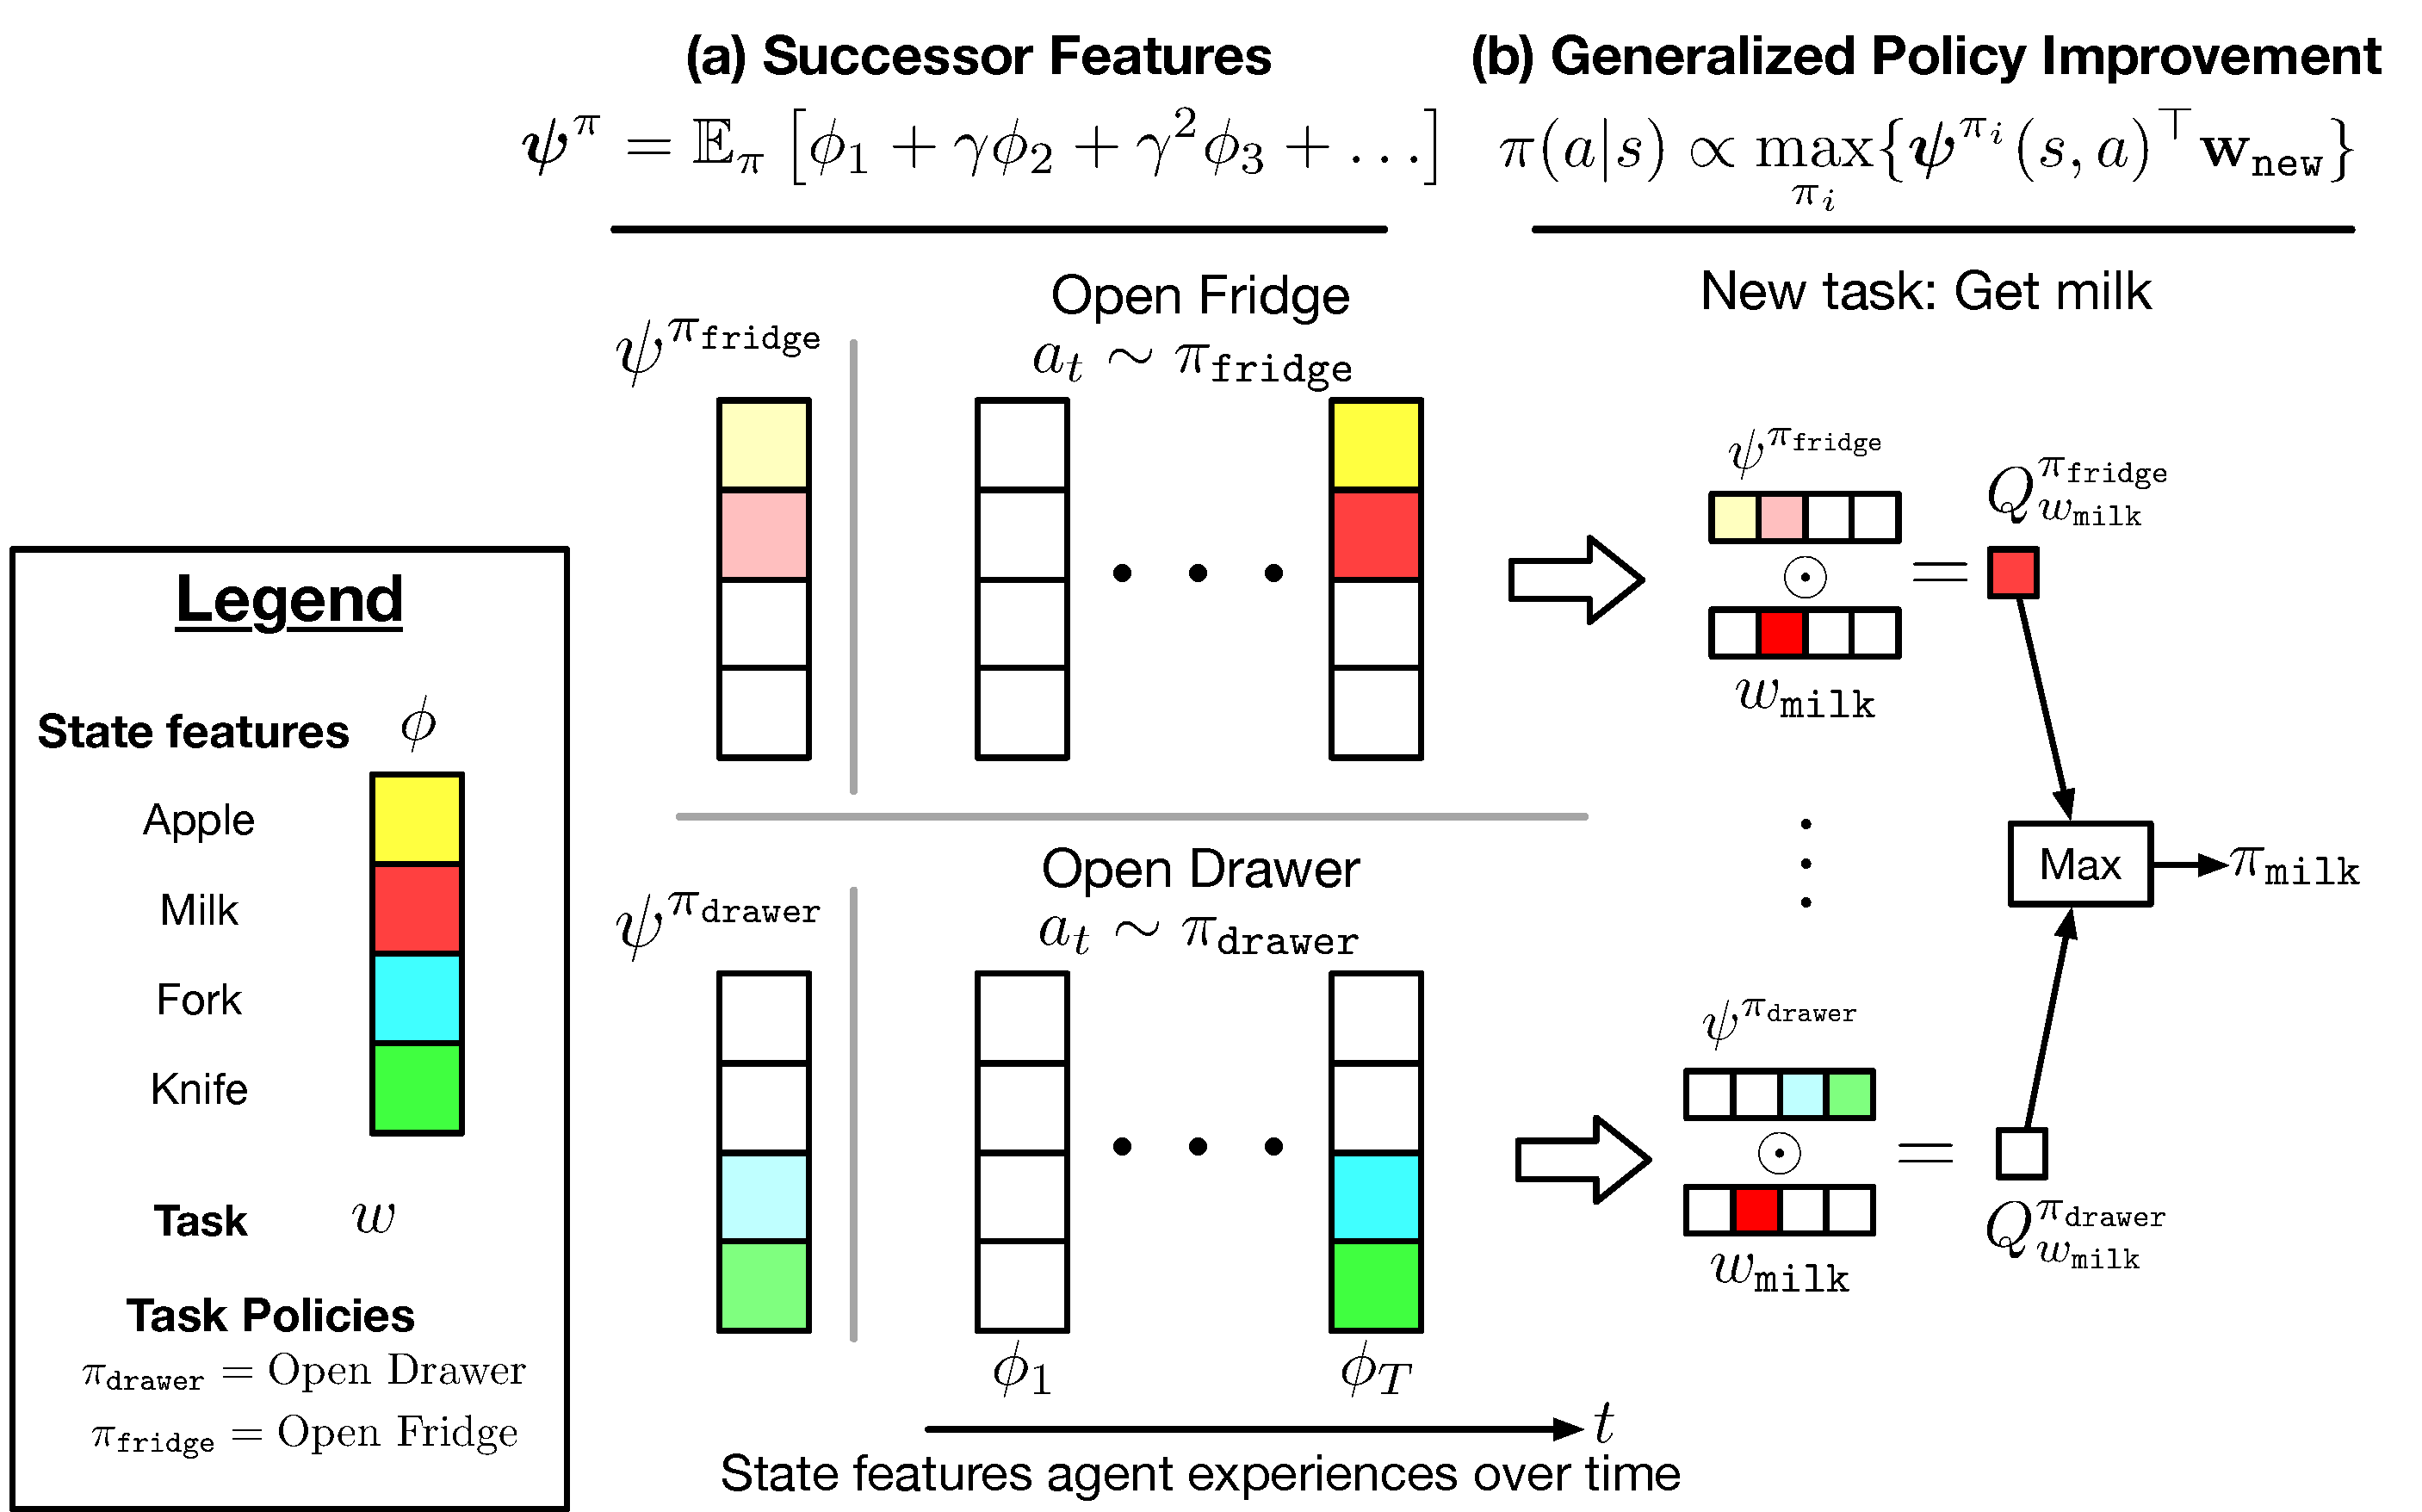
\includegraphics[height=3in]{figs/successor-features}
\caption{
  Illustration of successor features representation.
  (a)
  Here $\vphi_t=\vphi(s_t)$ is the vector of features
  for the state at time $t$, and $\vpsi^{\pi}$
  is the corresponding SF representation, which depends
  on the policy $\pi$.
  (b) Given a set of existing policies and their SFs,
  we can create a new one by specifying a desired
  weight vector $\wnew$ and taking a weighted combination
  of the existing SFs.
  \figtaken{Figure 5 of \citep{Carvalho2024}}.
    \figthanks{Wilka Carvalho}.
}
\label{fig:successorFeatures}
\end{figure}

Suppose we have learned a set of $N$ (potentially optimal)
policies $\pi_i$ and their corresponding SFs $\vpsi^{\pi_i}$
for maximizing rewards defined by $\vw_i$.
When presented with a new task $\wnew$,
we can compute a new policy using GPI as follows:
\begin{align}
  a^*(s;\wnew) &=
  \argmax_a \max_i Q^{\pi_i}(s,a,\wnew)
  =\argmax_a \max_i \vpsi^{\pi_i}(s,a)^\trans \wnew
\end{align}
If $\wnew$ is in the span of the training tasks
(i.e., there exist weights $\alpha_i$ such that $\wnew \sum_i \alpha_i \vw_i$),
then the GPI theorem states that $\pi(a|s)=\ind{a=a^*(s,\wnew)}$
will perform at least as well as any of the existing policies,
i.e., $Q^{\pi}(s,a) \geq \max_i Q^{\pi_i}(s,a)$
(c.f.,  policy improvement in \cref{sec:policyImprovement}).
See \cref{fig:successorFeatures} for an illustration.

Note that GPI is a model-free approach to computing a new policy,
based on an existing library of policies.
In \citep{Alegre2023}, they propose an extension that can also
leverage a (possibly approximate) world model to learn
better policies that can outperform the library
of existing policies by performing more decision-time search.


\subsubsection{Option keyboard}

One limitation of GPI is that it requires that the reward
function, and the resulting policy, be defined in terms of a fixed
weight vector $\wnew$, where the preference over features
is constant over time. However, for some tasks we might
want to initially avoid a feature or state and then later move
towards it.
To solve this, 
\citep{Barreto2019,Barreto2020} introduced the \keywordDef{option keyboard},
in which the weight vector for a task can be computed
dynamically in a state-dependent way, using
$\vw_s = g(s,\wnew)$.
(Options are discussed in \cref{sec:options}.)
Actions can then be chosen as follows:
\begin{align}
  a^*(s;\wnew) &=
    \argmax_a \max_i \vpsi^{\pi_i}(s,a)^\trans \vw_s
\end{align}
Thus the policy $\pi_i$ that is chosen  depends
in the current state. Thus $\vw_s$ induces a set of policies
that are active for a period of time, similar to playing
a chord on a piano.

%\subsubsection{Discovering cumulants}




\subsubsection{Learning SFs}

A key question when using SFs is how to learn the cumulants
or state-features
$\vphi(s)$.
Various approaches have been suggested,
including leveraging meta-gradients \citep{Veeriah2019},
image reconstruction \citep{Machado2018eigen},
and
maximizing the mutual information between task encodings
and the cumulants that an agent experiences when pursuing that task
\citep{Hansen2019}.
The cumulants are encouraged to satisfies the linear reward
constraint by minimizing
\be
\loss_r = ||r-\vphi_{\vtheta}(s)^\trans \vw||_2^2
\ee

Once the cumulant function is known,
we have to learn the corresponding SF.
The standard approach learns a different SF for every policy,
which is limiting. In \citep{Borsa2019} they introduced
\keywordDef{Universal Successor Feature Approximators}
which takes an input a policy encoding $\vz_{\vw}$,
representing a policy $\pi_{\vw}$ (typically we set $\vz_{\vw}=\vw$).
We then define
\be
\vpsi^{\pi_{\vw}}(s,a) = \vpsi_{\vtheta}(s,a,\vz_{\vw})
\ee
The GPI update then becomes
\be
a^*(s;\wnew) = \argmax_a \max_{\vz_{\vw}} \vpsi_{\vtheta}(s,a,\vz_{\vw})^\trans \wnew
\ee
so we replace the discrete max over a finite number of policies
with a continuous optimization problem (to be solved per state).

If we want to learn the policies and SFs at the same time,
we can optimize the following losses in parallel:
\begin{align}
  \loss_Q &= ||\vpsi_{\vtheta}(s,a,\vz_w)^\trans \vw - \vy_Q||,
  \;
  \vy_Q = R(s';\vw) + \gamma \vpsi_{\vtheta}(s',a^*,\vz_w)^\trans \vw
  \label{eqn:LQ} \\
  \loss_{\vpsi} &= ||\vpsi_{\vtheta}(s,a,\vz_{\vw}) - \vy_{\vpsi}||,
  \;
  \vy_{\vpsi} = \vphi(s') + \gamma \vpsi_{\vtheta}(s',a^*,\vz_{\vw})
\end{align}
where $a^* = \argmax_{a'} \vpsi_{\vtheta}(s', a', \vz_{\vw})^\trans \vw$.
The first equation is standard Q learning loss,
and the second is the TD update rule
in \cref{eqn:SFTD} for the SF.
In \citep{Carvalho2023}, they present the
\keywordDef{Successor Features Keyboard},
that can learn the policy,
the SFs 
and the task encoding $\vz_{\vw}$,
all simultaneously.
They also suggest replacing the squared error regression
loss in \cref{eqn:LQ} with a cross-entropy loss,
where each dimension of the SF is now a
discrete probability distribution
over $M$ possible values of the corresponding feature.
(c.f. \cref{sec:classifRL}).


\subsubsection{Choosing the tasks}

A key advantage of SFs is that they provide a way
to compute a value function and policy for any given reward,
as specified by a task-specific weight vector $\vw$.
But how do we choose these tasks?
In \citep{Hansen2019} they sample $\vw$ from a distribution
at the start of each task, to encourage the agent
to learn to explore different parts of the state space
(as specified by the feature function $\vphi$).
In \citep{Liu2021} they extend this by adding an intrinsic
reward that favors exploring parts of the state space
that are surprising (i.e., which induce high entropy),
c.f., \cref{sec:intrinsicReward}.
In \citep{Farebrother2023}, they introduce
\keywordDef{proto-value networks},
which is a way to define auxiliary tasks based on  successor
measures.

\eat{
\subsection{Forwards-backwards representations: TODO}
\label{sec:FB}

\citep{Touati2021,Touati2023}
}


%%%%%%%%%%%


\eat{
\subsection{Predictive state representations}
\label{sec:PSR}

An alternative to working with belief states
is to  marginalize out the POMDP
latent state $z_t$,
to derive a set of predictions over future observables $\vo_{t+1:T}$
as a function of the past history of observables, $\vh_t$,
and future actions, $\va_{t+1:T}$.
This can then become a learning  target for a model, that is trained
to directly
predict  future observations, without explicitly invoking the concept
of latent state.
This is called a \keywordDef{predictive state representation}
or \keywordDef{PSR} \citep{PSR}.
This is related to the idea of
\keywordDef{observable operator models}
\citep{Jaeger2000}.
See also \cref{sec:SR} where we discuss successor representations.
%However, it is not clear which features of the future observables
%are worth modeling.
%(GVFs, discussed in \cref{sec:GVF}, share the same problem.)
}


\eat{
\subsection{General value functions}
\label{sec:GVF}

So far we have mainly been focused on predicting the sum of expected
discounted future rewards, i.e., the value function.
But the reward is just one possible signal of interest we can extract from the environment.
We can generalize this by considering a \keywordDef{cumulant}
$C_t \in \real$, which is some scalar of interest derived from the observation
(e.g., did a loud bang just occur? is there a tree visible in the image?).
We then define the \keywordDef{general value function} or \keywordDef{GVF}
as follows \citep{GVF}:
\be
V_{\pi,\gamma,C}(s) = \expect{
  \sum_{k=t}^{\infty} \left(\prod_{i=t+1}^k \gamma(S_i) \right)
  C_{k+1} \vert S_t=s, A_{t:\infty} \sim \pi}
\ee
where $1-\gamma(s)$ is the probability of terminating in state $s$.
If we set $C(s)=R(s)$ and $\gamma(s)=\gamma$, we recover the value function.
But we can use the GVF to predict the probability of
other \keywordDef{auxiliary tasks}, such as the occurence of a loud bang;
and unlike a standard one-step predictive model,
we don't need to know exactly when the event will occur.
(See also \citep{Ring2021}.)

By training a model to compute GVFs for multiple related cumulants,
we can  learned a useful state representation more efficiently than just
learning from the reward by itself, while still avoiding the need
to reconstruct the entire observation.
Thus this is a form of non-generative world model,
as discussed in \cref{sec:MBRLnongen}.
The benefits of this kind of approach were shown in
\citep{Jaderberg2017iclr}.


Note that training GVFs using some kind of TD learning
is inherently an off-policy learning problem, since the data is being
collected by a policy to maximize reward, but the other cumulants
are just being predicted, not maximized.
Since the GVF is typically a neural network with multiple output heads,
we need to tackle the \keyword{deadly triad}, which we discussed in 
\cref{sec:deadlyTriad}.
One approach is to use gradient TD methods, which are provably convergent.
This has been applied to GVF learning in \citep{Xu2022GVF}.
However, the question of which cumulants are worth learning is still open.
}

